
%!TEX root=../2022_IEEE_DEB_Vizier.tex

% %%%%%%%%%%%%%%%%%%%%%%%%%%%%%%%%%%%%%%%%
% \begin{figure}[t]
%   \centering
%   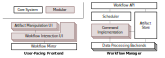
\includegraphics[width=0.7\textwidth]{graphics/systemarch}\\[-5mm]
%   \caption{Vizier's architecture, comprised of a user-facing frontend component and a backend component.}\label{fig:vizier-architecture}
% \end{figure}
% %%%%%%%%%%%%%%%%%%%%%%%%%%%%%%%%%%%%%%%%

%%%%%%%%%%%%%%%%%%%%%%%%%%%%%%%%%%%%%%%%%%%%%%%%%%%%%%%%%%%%%%%%%%%%%%%%%%%%%%%%
\pagebreak[4]
\subsection{Solution Overview}
\label{sec:solution-overview}

%%%%%%%%%%%%%%%%%%%%%%%%%%%%%%%%%%%%%%%%
\begin{wrapfigure}[12]{r}[0pt]{12cm}
  \centering
  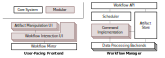
\includegraphics[width=0.7\textwidth]{graphics/systemarch}\\[-5mm]
  \caption{Vizier's architecture, comprised of a user-facing frontend component and a backend component.}\label{fig:vizier-architecture}
\end{wrapfigure}
%%%%%%%%%%%%%%%%%%%%%%%%%%%%%%%%%%%%%%%%
An overview of Vizier's architecture is shown in \Cref{fig:vizier-architecture}.
Addressing requirement \textbf{W1}, the central abstraction in Vizier is a workflow: a linear sequence of steps. % taken by the user in pursuit of a specific objective.
Unlike classical workflow systems, Vizier does not require users to explicitly declare information flow between steps.
Rather Vizier borrows the model employed in popular computational notebooks like Jupyter, where inter-cell communication occurs through a global state (artifacts) passed sequentially through steps.
Following notebook conventions, we refer to these steps as \emph{cells}, and the global state as a \emph{scope}, a map from artifact name to the version of the artifact valid at this point in the workflow. Vizier stores artifacts in common formats through a versioned \textbf{Artifact Store} (\Cref{sec:data-artifacts}), addressing requirement \textbf{A2}.
In \Cref{sec:vizier-workflows}, we formalize Vizier's workflow model, and show how we satisfy requirement \textbf{W3} by instrumenting how each cell interacts with the scope, allowing us to determine what artifact versions are valid.

Vizier's workflow semantics, paired with the versioned artifact store and workflow versioning (\Cref{sec:vizier-history}) addresses requirement \textbf{W2}. % as notebooks have a natural concept of logical order (the order of cells in the notebook) that can be adjusted over time.
% Adding workflow versioning  is sufficient to fully address the requirement.
In contrast, classical notebooks like Jupyter or Zeppelin rely on the global state of an interpreter for inter-cell communication.
Reverting this state to an earlier revision is challenging~\cite{zelnicki:2017:nodebook}, limiting their ability to satisfy requirement \textbf{W3}.
Vizier instead relies on its versioning system, allowing its \textbf{Scheduler} to automatically detect and re-evaluate stale cells (\Cref{sec:vizier-scheduler}).
To address requirement \textbf{A3}, we designed a light-weight uncertain data model that is implemented in Vizier in the form of \textit{caveats}, annotations on data that indicate uncertain values and rows  (\Cref{sec:data-docum-error}).

Addressing requirement \textbf{A1} requires modularity in both Vizier's front- and back-end components.
First, the user's interactions with a workflow and artifacts, whether through a scripting language, graphical interaction, or any other modality, need to be captured for replay (simultaneously addressing requirement \textbf{A4}). In Vizier this is achieved by requiring that every update to an artifact made through a particular modality has to be reflected as an operation in the workflow, i.e., a data update is translated into a workflow update.
Vizier manages a collection of \textbf{Command Implementations} that implement the logic behind these artifact transformations (\Cref{sec:multimodality}).
To streamline the implementation of commands, Vizier's data formats and transformations are built over standard \textbf{Data Processing Backends} like Apache Spark.
% For example, Vizier supports fine-grained provenance over datasets by encoding them as Spark data frames.

The frontend is implemented over a \textbf{Workflow Mirror} that uses websockets to reflect a live view of the workflow the user is editing.
Vizier automatically derives a default \textbf{Artifact Manipulation User Interface} for its notebook interface from each command's parameter schemas. This interface suffices for many templated commands, but the frontend can be further extended to provide a more customized experience, for example for Spreadsheet-style direct manipulation of data (\Cref{sec:spreadsheets}).
As illustrated in \Cref{fig:screenshot}, the frontend displays three \textbf{Workflow Interaction User Interfaces} by default: (i) A direct display of the workflow as a notebook, (ii) a table of contents summary of the notebook, including highlighting from documentation, and (iii) a list of artifacts derived by the notebook.
Several of these components, including the notebook and the artifact list provide access to direct manipulation interfaces.
Additional views currently implemented in Vizier include: (iv) A caveat view (\Cref{sec:data-docum-error}) that shows and tracks potential errors in the workflow and data, (v) a history view that shows the evolution of the workflow over time, and (vi) a data provenance subway diagram view.

%%%%%%%%%%%%%%%%%%%%%%%%%%%%%%%%%%%%%%%%%%%%%%%%%%%%%%%%%%%%%%%%%%%%%%%%%%%%%%%%
\begin{figure}
  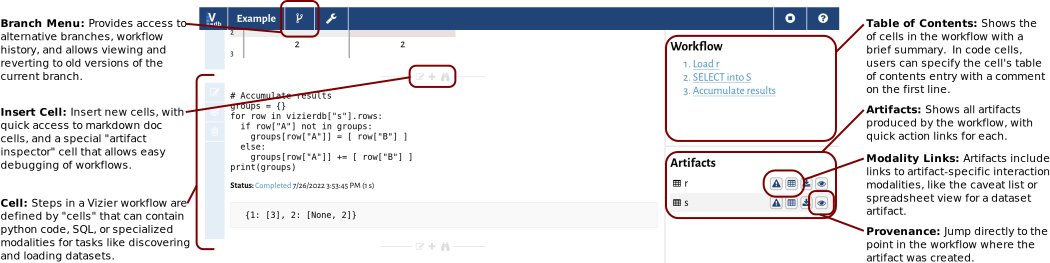
\includegraphics[width=\textwidth]{graphics/screenshot.pdf} 
  \caption{The Vizier User Interface}
  \label{fig:screenshot}
\end{figure}
%%%%%%%%%%%%%%%%%%%%%%%%%%%%%%%%%%%%%%%%%%%%%%%%%%%%%%%%%%%%%%%%%%%%%%%%%%%%%%%%

%%% Local Variables:
%%% mode: latex
%%% TeX-master: "../2022_IEEE_DEB_Vizier"
%%% End:


\section{Method}

% \vspace{-3mm}
\GraphEval{} is designed to measure the factuality of a language model in relation to a \cz{KG}. As presented in Figure \ref{fig:framework}, the proposed work is divided into three steps: 
\begin{itemize}[topsep=0pt,itemsep=0pt,parsep=0pt,partopsep=0pt,leftmargin=*]
    \item \textbf{Step 1: Question and label collection from KGs and LLMs. } \quad  The model samples triples from KGs and converts each triple into a declarative statement with GPT-4-crafted templates. To prepare versatile statements, we employ \textit{negative sampling}, where incorrect statements are intentionally generated. Afterward, those statements are posed to collect the labels answered by an LLM (i.e., Yes, No, and I don't know (IDK)).
    \item \textbf{Step 2: Judge model training.} \quad With the triples collected in the first step, we train a judge model to avoid long-generated texts and conserve computational resources. In detail, inspired by~\cite{azaria-mitchell-2023-internal}, we train a classifier with LLMs' hidden states to make a selection within the above three options. We also apply p-tuning \cite{liu2021p} to minimize the prompt/instruction size.
    \item \textbf{Step 3: Evaluation on whole KGs.} \quad Similar to the first step, we retrieve all true/false statements from KGs. Subsequently, these statements are fed into the trained judge model to estimate the factuality of LLM. This process enables a thorough and multifaceted analysis of the LLM's performance in terms of factuality, drawing from a wide range of perspectives to provide a more comprehensive and diversified evaluation.
\end{itemize}
In the following sections, we will discuss the details of each step. 

\subsection{Question and Label Collection}
\label{sec:question_generation}

\paragraph{Question Generation}
In order to evaluate the language model's ability to identify false statements, we directly construct a declarative sentence for each triple. This addresses the ineffectiveness of multiple-choice questions in our task. %
Firstly, multiple-choice prompts may cause misalignment with parametric knowledge in LLMs. Since LLMs mainly learn parametric knowledge through text data, in which knowledge facts are mostly represented as declarative sentences~\cite{weller2023according}, employing multiple-choice questions may hinder the evaluation of factuality. Secondly, multiple-choice questions have more complex labels (i.e. A, B, C, D) than declarative sentences (i.e. True, False, IDK), which can complicate the tasks for the judge model, influencing the overall effectiveness. We use an example to illustrate this.

\begin{examplethm}
    For the triple \texttt{(Barack Obama, birthPlace, Hawaii)}, a multi-choice question can be generated as \texttt{Where was Barack Obama born?} with choices \texttt{A. Hawaii B. Chicago C. New York D. Los Angeles}. Here, for the same triple, we can also generate another multi-choice question as \texttt{Where was Barack Obama born?} with choices \texttt{A. China, B. Hawaii, C. Japan, D. Russia}. The two questions represent the same triple, but the choices are different. %
    As mentioned in the last paragraph, this can introduce complexity and potential misalignment with an LLM’s training and result in inconsistent responses. %
    
\end{examplethm}

To address the ineffectiveness of multiple-choice questions, we propose to directly ask the LLMs whether a statement is true or not.
For instance, considering the triple \texttt{(Barack Obama, birthPlace, Hawaii)}, we can formulate a fact \texttt{Obama was born in Hawaii} by integrating the entities \texttt{Barack Obama} and \texttt{Hawaii} into the template \texttt{ \{head\} was born in \{tail\}}. %
Each template corresponds to the relation of a triple, and they are crafted to be clear and straightforward statements. GPT-4 is employed to generate these templates for all relations in the \cz{KG}. 
 These generated templates are then manually reviewed and refined to ensure their compatibility with the \cz{KG}. Then, we can ask a question to the LLMs, such as \texttt{Is the statement "Barack Obama was born in Hawaii" true or false?}.
    Here, the templates are corresponding to the relations of the triples. This is because the number of relations in the \cz{KG} is limited, while the number of triples is large. Therefore, we can use the relations to categorize the triples, and then use the templates to generate questions for each category. This can significantly reduce human labor, i.e., monitoring less than 1000 templates compared with monitoring more than 10 million triples.
See the Appendix~\ref{app:detailed_settings} for the detailed settings of the relation templates.

\paragraph{Negative sampling}
Although the declarative sentences simplify the training of the judge model, they alone are insufficient to evaluate the language model's factual accuracy. LLMs can simply answer true for every question, and still get a high accuracy. %
To address this, we introduce negative sampling, a technique commonly used in \cz{KG} completion tasks, to generate false statements. Specifically, we randomly replace one entity or relation in the original triple with another entity or relation sampled from the \cz{KG}. For example, given the triple \texttt{(Barack Obama, birthPlace, Hawaii)}, we can replace the tail entity \texttt{Hawaii} with another entity \texttt{Chicago} to form the false statement \texttt{Barack Obama was born in Chicago}. These false statements are then presented to the LLMs to evaluate their ability to identify falsehoods.

\vspace{-2mm}
\subsection{Judge Model}\label{method:judge}

% \vspace{-2mm}
% \wfj{\paragraph{Motivations} }

\vspace{-2mm}
Normally, to evaluate the factual accuracy of a language model, we would generate questions from a \cz{KG} and then pose these questions to the language model. However, given the expansive nature of \cz{KG}s, it's impractical to label every generated question by the LLM. 
A more efficient approach is to use the last token logits of the LLMs as their answers. However, %
recent research has highlighted discrepancies between these logits and the model's actual text outputs~\cite{wang2024myanswer}. 
Therefore, we introduce a novel judge model to assist with this task. The judge model, initially trained on a subset of labeled questions, is then employed to label the remaining questions. Uniquely, inspired by ~\cite{azaria-mitchell-2023-internal}, the judge model utilizes the LLM's hidden state as input, as a replacement of the LLM's last layer with compressed output tokens. Specifically, three output classes are used: \textit{True}, \textit{False}, and \textit{I don't know}. The judge model is a two-layer feed-forward neural network, with a layer normalization and a ReLU activation function. 
This approach diverges from standard practices where LLMs generate answers, as here we only forward the transformer once. Consequently, this operation is significantly less resource-intensive than full answer generation, allowing the judge model to efficiently process a large number of questions with limited labeled data.
% \vspace{-2mm}
\wfj{With this model, we can glance at the correctness of an LLM, i.e., how likely the model can answer a question relevantly and correctly. We evaluate the performance of the judge model using two metrics: (i) \textit{Truthfulness}, i.e., the likelihood that the judge model prediction matches the LLM correctness under a given question; and (ii) \textit{Informativeness}, i.e., the likelihood that the judge model does not give a prediction of `I don't know.' 
% Clarifying question on Page 5: Why were "truthfulness," "informativeness," and "correctness" prioritized over other possible metrics like "relevance"? OR “correctness” is like “relevance”?
Since the evaluation is based on a general KG that spans multiple domains, other metrics such as ``Relevance'' would typically require a more specific contextual framework. Nonetheless, future research could explore the use of more context-specific metrics tailored to the LLM's domain of application.
}

\vspace{-2mm}
\paragraph{Efficiency}
To further enhance the judge model's efficiency, we include 2 extra components. First, we found that the instruction prefix of the LLMs is too large for the judge model to process efficiently. We thus fine-tune a {\it prompt encoder}~\cite{liu-etal-2022-p} to reduce the large input of the prompt prefix, which would be the same for all questions. 
Second, we found that our judge model, with the training process on the labeled dataset, is robust to the LLM's hidden states. %
In experiments, we observed that our judge model can seamlessly utilize hidden states from distinct LLMs without significant differences in performance. For instance, within the LLaMA 2 model family, which contains 3 models with different parameters: 7B, 13B, and 70B, we found that the judge model's performance is consistent regardless of whether the hidden states are from 7B, 13B, or 70B. %
Therefore, we can use the model with the least parameters, as a {\it substitute model} when computing the hidden states. This gives us a huge reduction in computational cost.






\paragraph{Analysis of Judge model}
In this part, we assume there are two datasets; one is for training the judge model, and the other is for evaluation, denoted by $\mathcal{D}_S$ and $\mathcal{D}_T$, respectively. As the proposed judge model leads to a triple classification task, we assume a hypothesis portfolio $h = \{h_t, h_f, h_{idk}\}$, where these three hypotheses separately predict if a sample can be correctly answered by the LLM, i.e., True, False, and IDK. In other words, the hypothesis $\hat{h} \in h$ maps an input $\mathbf{x}$ to $\{0, 1\}$, where $1$ means the input satisfies the hypothesis conditions. For a given input $\mathbf{x}$, the equality 
$h(\mathbf{x}) = h_t(\mathbf{x}) + h_f(\mathbf{x}) + h_{idk}(\mathbf{x}) = 1$
always holds because the judge model provides an only output. Define the convex loss function for a hypothesis $\hat{h} \in h$ to be $$L_{\mathcal{D}}(\hat{h}) = \sum_{(\mathbf{x}, y) \in \mathcal{D}} |\hat{h}(\mathbf{x}) - \boldsymbol{1}_{\hat{h}}(y)|,$$ where $\boldsymbol{1}_{\hat{h}}(y)$ indicates if the data indeed satisfies the hypothesis. Since a wrong prediction for data $(\mathbf{x}, y)$ results in $\sum_{\hat{h} \in h} |\hat{h}(\mathbf{x}) - \boldsymbol{1}_{\hat{h}}(y)| = 2$, we define the misclassification rate as 
$$L_{\mathcal{D}} \left(h\right) = \frac{1}{2} \left(L_{\mathcal{D}} \left(h_t\right) + L_{\mathcal{D}} \left(h_f\right) + L_{\mathcal{D}} \left(h_{idk}\right)\right) $$ 

Below is a theoretical analysis to understand the bound of the misclassification rate, which is driven by Theorem 2 of \cite{ben2010theory}.

\begin{theoremthm}
Let $\mathcal{H} = \{\mathcal{H}_t, \mathcal{H}_f, \mathcal{H}_{idk}\}$ be a set of hypothesis spaces of VC dimension $d$. If $\mathcal{U}_S, \mathcal{U}_T$ are the samples of size $m$ each, drawn from $\mathcal{D}_S$ and $\mathcal{D}_T$, respectively, then for any $\delta \in (0, 1)$, with probability at least $1-\delta$, for every $h \in \mathcal{H}$, we have
\begin{equation}
    L_{\mathcal{D}_T} \left(h\right) \leq L_{\mathcal{D}_S} \left(h\right) + \frac{3}{4} d_{\mathcal{H} \Delta\mathcal{H}} \left(\mathcal{U}_S, \mathcal{U}_T\right) + 6 \sqrt{\frac{2d \log \left(2m\right) + \log\left(2/\delta\right)}{m}} + \frac{1}{2} \lambda
\end{equation}
where $\lambda = \inf_{h \in \mathcal{H}} \left(L_{\mathcal{D}_S}\left(h\right) + L_{\mathcal{D}_T}\left(h\right)\right)$ is the optimal combined error, $d_{\mathcal{H} \Delta\mathcal{H}}$ measures the distribution discrepancy between two distributions. 
\end{theoremthm}
\feijie{The above theorem provides insights for the generalization bound of the judge model. The bound is associated with the discrepancy between training data $\mathcal{D}_S$ and evaluation data $\mathcal{D}_T$, and the discrepancy can be measured by drawing samples from both training and evaluation datasets for an equivalent size. Moreover, the bound is affected by the optimal hypothesis over all the data, i.e., $\mathcal{D}_S \cup \mathcal{D}_T$, where a lower error leads to improved performance of the judge model.}



\subsection{Evaluation}


For evaluating the LLM's performance, we consider \textit{Correctness}, which is defined as the proportion of questions for which the LLM's response matches the true label (or false label if the question is generated from a negative triple). This captures the accuracy of the LLM in identifying correct information and distinguishing it from fabricated (negative) triples.
We also adopt the metrics of \textit{Truthfulness} and \textit{Informativeness}, as defined in \cite{TruthfulQA}. \textit{Truthfulness} refers to the likelihood of the language model (LLM) providing an honest response. A response is considered \Truthful{} if the LLM either provides the correct answer or opts for `I don't know'. This criterion assesses the model's ability to be honest about what it knows and to admit uncertainty rather than making false statements. \textit{Informativeness} is the probability of the LLM offering any substantive information, irrespective of its accuracy. An answer is deemed \Informative{} if it is anything other than `I don't know'. This reflects the model's capacity to provide substantial information without resorting to uncertainty or avoidance of an answer. 

When considering multiple negative triples sampled, we combine the results for all negative triples sampled from a triple $\tau$, as well as the results for their original positive triple $\tau$, to calculate the overall performance of the LLM. 
Since correctly detecting a real triple from KG is much simpler than detecting a negative triple, we want to give a max penalty to the LLM's wrong response to the real triple when designing the metric. Therefore, if a real triple is predicted as false, the LLM will score $0$ across all metrics. Then, the negative triple results are averaged to give a fine-grained evaluation of the LLM's performance.
To achieve this, for each performance metric, we define functions $\mathcal{F}$ which evaluates the LLM's response to $\tau$ and $\mathcal{F}'$  to each negative triple $\tau'$ sampled from $\tau$. The overall performance metric for $\tau$ is then calculated as:
\begin{equation}
\text{Metric}(\tau) = \max\left(0, \mathcal{F}(\tau) - \frac{1}{|\mathcal{N}(\tau)|}
\sum_{\tau' \in \mathcal{N}(\tau)} \mathcal{F}'(\tau')\right)
\end{equation}
Here, $\mathcal{N}(\tau)$ represents the set of all negative triples generated from the positive triple $\tau$. $\mathcal{F}$  and $\mathcal{F}'$ are defined as follows: \cz{\textbf{\textit{(\rmnum{1})}}} {\it Correctness.}
    $\mathcal{F}$ is defined such that it is $1$ if the judge model predicts that a real (positive) triple is True, and it is $0$ otherwise; $\mathcal{F}'$ is 0 if the judge model predicts a negative triple as False, and 1 otherwise. 
    \cz{\textbf{\textit{(\rmnum{2})}}} {\it Truthfulness.}
    When measuring \textit{Truthfulness}, $\mathcal{F}$ is set to $1$ if the judge model's prediction for the input $\tau$ is either True or IDK, and it is $0$ otherwise. Similarly, $\mathcal{F}'$ is set to $1$ if the judge model's prediction for the input $\tau'$ is True, and $0$ otherwise; and 
    \cz{\textbf{\textit{(\rmnum{3})}}} {\it Informativeness.}
    For \textit{Informativeness}, $\mathcal{F}$ is defined as $1$ if the judge model's prediction for the input $\tau$ is anything other than "I don't know", and it is $0$ otherwise. $\mathcal{F}'$ is set to $1-\mathcal{F}$ on the informativeness metric.
By applying this equation, we can systematically compute the \textit{Correctness}, \textit{Truthfulness}, and \textit{Informativeness} of an LLM's responses in a consistent and comprehensive manner, offering a detailed insight into its overall performance. 



 













